\begin{appendices}

\section{Meijer's G-function}\label{sec:Meijer_G_functions}

Recall that $\Gamma(z)$ denotes the Gamma function. Let $p, q, m, \ell$ be four integers satisfying $0 \le m \le q$ and $0 \le \ell \le p$ and consider two sequences ${\bf a}_p = \{a_1, \dots, a_p\}$ and ${\bf b}_q = \{b_1, \dots, b_q\}$ of reals such that $a_i - b_j$ is not a positive integer for all $1 \le i \le p$ and $1 \le j \le q$ and $a_i - a_j$ is not an integer for all distinct indices $1 \le i, j \le p$. Then, with $\iota$ denoting the complex unit, Meijer's G-Function~\cite{meijer1946g} is defined as
\begin{equation}\label{eq:def_Meijer_G_function}
	\MeijerGnew{m}{\ell}{p}{q}{{\bf a}}{{\bf b}}{z} 
	= \frac{1}{2 \pi \iota} \int_L 
	\frac{\prod_{j = 1}^{m}\Gamma(b_j - t) \prod_{j = 1}^\ell \Gamma(1 - a_j + t)}
	{\prod_{j = m + 1}^{q}\Gamma(1 - b_j + t) \prod_{j = \ell + 1}^p\Gamma_n(a_j-t)} \, z^t \dd t,
\end{equation}
where the path $L$ is an upward oriented loop contour which separates the poles of the function $\prod_{j = 1}^{m}\Gamma(b_j - t)$ from those of $\prod_{j = 1}^n \Gamma(1 - a_j + t)$ and begins and ends at $+\infty$ or $-\infty$.

The Meijer's G-Function is of a very general nature and has relation to many known special functions such as the Gamma function and the generalized hypergeometric function. For more details, such as many identities for $\MeijerGnew{m}{\ell}{p}{q}{{\bf a}}{{\bf b}}{z}$ see \cite{gradshteyn2015table,luke2014mathematical}.

For our purpose we need the following identity which follows from an Mellin transform operation.

\begin{lemma}
For any $a\in \R$ and $\xi, s>0$,
$$\Gamma^+(-a-1,\xi/s) = \MeijerGnew{2}{0}{1}{2}{1}{-a-1,0}{\frac{\xi}{s}}$$
\end{lemma}
\begin{proof}
Let $x>0$ and $q\in\R$ and note that as the $\Gamma$-function is the Mellin transform of $e^{-x}$, by the inverse Mellin transform formula, we have $e^{-x}=\frac{1}{2\pi i}\int_{c-i\infty}^{c+i\infty} \Gamma(p)x^{-p}dp$ for $c>0$ (see \cite[p.196]{davies2012integral}). Applying the change of variable $p(r)=q-r$ yields $e^{-x}=\frac{1}{2\pi i}\int_{c+q-i\infty}^{c+q+i\infty} \Gamma(q-r) x^{r-q}dr$, then multiplying both sides with $-x^{q-1}$ gives $-x^{q-1}e^{-x} = -\frac{1}{2\pi i}\int_{c+q-i\infty}^{c+q+i\infty} \Gamma(q-r) x^{r-1}dr$. Now, integrating both sides gives $\int_x^\infty t^{q-1}e^{-t}dt = \frac{1}{2\pi i}\int_{c+q-i\infty}^{c+q+i\infty}\frac{\Gamma(q-r)}{-r}x^r dr$. On the left-hand side is the incomplete gamma function and on the right-hand side with using $-r= \frac{\Gamma(1-r)}{\Gamma(-r)}$ is the Meijer $G$-function, i.e. $\Gamma^+(q,x)=\MeijerG{2}{0}{1}{2}{1}{q,0}{x}$. The claim follows by plugging in $q=-a-1$ and $x=\frac{\xi}{s}$.
\end{proof}

\section*{Properties of $G_{\H,n}(\alpha,\nu)$}

\PvdH{@Markus: is the lemma below only needed to prove the second lemma? If so than we can remove it because the statements of the second lemma have already been established in other parts of the paper.}

\begin{lemma}[Intensity measure of the intersection of two neighbourhood balls]\label{lem:mu3}
Consider the Poisson hyperbolic random graph conditioned on having two vertices with degree $k$ at heights $y_1, y_2 \in [y_{k,-},y_{k,+}]$ and horizontal distance $d$. Then the expected number of vertices in the intersection of their neighbourhood balls in the infinite limit model is $\Theta(k^{2\alpha}d^{1-2\alpha})$.
\end{lemma}
\begin{proof}
Denote the two vertices by $v$ and $w$.
If the neighbourhood balls of $v$ and $w$ intersect at the minimal height $y_h$, then $d = e^{\frac{y_h+y_1}{2}}+e^{\frac{y_h+y_2}{2}}$.

Due to our assumption $y_1, y_2 \in [y_{k,-},y_{k,+}]$, this condition implies $d \leq 2 e^{\frac{y_h+y_{k,+}}{2}}$. This implies $y_h \geq 2\ln \frac{d}{2} - y_{k,+}$. (In a similar fashion, we infer that $y_h \leq 2\ln \frac{d}{2} -y_{k,-}$.)

Therefore, using $y_1,y_2 \in [y_{k,-}, y_{k,+}]$ and $e^{\frac{y_1}{2}}, e^{\frac{y_2 }{2}} \sim k$, $e^{\frac{y_h}{2}} \sim \frac{d}{k}$:
\begin{align*}
\mu_3 &= \int_{y_h}^\infty (e^{\frac{y_1+y}{2}}+e^{\frac{y_2+y}{2}} - d) \alpha e^{-\alpha y} dy =\Theta(k)\frac{\alpha}{\alpha-\frac{1}{2}} e^{(\frac{1}{2}-\alpha) y_h} +d e^{-\alpha y_h} \\
&= \Theta(k (\frac{d}{k})^{1-2\alpha} +d(\frac{d}{k})^{-2\alpha}) = \Theta(k^{2\alpha} d^{1-2\alpha})
\end{align*}
\end{proof}

The following proposition establishes several properties on the number of vertices with degrees $k_n$ in the Poisson hyperbolic graph $G_{\widetilde{\H},n}(\alpha,\nu)$.

\begin{proposition}
Let $\alpha > \frac{1}{2}$, $\nu > 0$, consider the Poisson hyperbolic random geometric graph $G_{\widetilde{\H},n}(\alpha,\nu)$ and let $N_{\widetilde{\H},n}(k_n)$ be the number of degree $k_n$ vertices.
\begin{enumerate}
	\item If $2 \leq k_n \leq n-1$ such that $k_n \rightarrow \infty$ as $n \rightarrow \infty$, then $\E[N_{\widetilde{\H},n}(k_n)] \sim 2\alpha \xi^{2\alpha} n k_n^{-(2\alpha +1)}$ as $n \rightarrow \infty$.
	
	\item In particular if $k_n \gg n^{\frac{1}{2\alpha+1}}$, then $N_{\widetilde{\H},n}(k_n) = 0$ w.h.p.
	
	\item Furthermore, if $k_n \ll n^{\frac{1}{2\alpha+1}}$, then $\frac{\E[N_{\widetilde{\H},n}(k_n)^2]}{\E[N_{\widetilde{\H},n}(k_n)]^2} \rightarrow 1$, so in particular in this case w.h.p. $$N_{\widetilde{\H},n}(k_n) = (1+o(1))\E[N_{\widetilde{\H},n}(k_n)]$$ and $N_{\widetilde{\H},n}(k_n) > 0$ w.h.p.
\end{enumerate}
\end{proposition}

\begin{proof}
\PvdH{The results from this lemma are already stated elsewhere but I kept the lemma to not break any references. It will be cleaned next round.}
	
%(i): First of all, we note that the degree of a vertex at height $y \in [0,R_n]$ is a Poisson random variable with expectation $\lambda_n(y) := \mu_{\alpha,\nu}(\BallHyp{y})$. As $N_{\widetilde{\H},n}(k_n) = \sum_{v\in V(G_{\widetilde{\H},n})} \1_{\{D_{\widetilde{\H},n}(v) = k_n\}}$, by the Palm-Mecke formula,
%\begin{align*}
%	\Exp{N_{\widetilde{\H},n}(k_n)} &= \int_{\Rcal_n} \Prob{D_{\widetilde{\H},n}(y) = k_n} 
%		f_{\alpha,\nu}(x,y) \dd x \dd y \\
%	&= n \int_0^{R_n} \Prob{D_{\widetilde{\H},n}(y) = k_n} \alpha e^{-\alpha y} \dd y 
%		= n \int_0^{R_n} \Prob{\Po(\lambda_n(y))=k_n} \alpha e^{-\alpha y}dy.
%\end{align*}
%
%Now, we would like to replace the $\mu_{y}^{(n)}$ in the Poisson probability above by $\xi e^{\frac{y}{2}}$. The argument for this splits into the following parts: $\mu_{y}^{(n)} \rightarrow \xi e^{\frac{y}{2}}$ as $n\rightarrow \infty$, together with the concentration resp. range of $y$, it follows that $\Pee(Po(\mu_y^{(n)})=k_n) \sim \Pee(Po(\xi e^{\frac{y}{2}})=k_n)$; finally the asymptotic equivalence of the integrands implies the asymptotic equivalence of the integrals. 
%
%The convergence of $\mu_{y}^{(n)}$ to $\xi e^{\frac{y}{2}}$ is by  Lemma \ref{lem:expecdeg}. \PvdH{I do not follow this argument. By Lemma \ref{lem:expecdeg}, for some fixed $\varepsilon > 0$,
%\[
%	\mu_y^{(n)} = \xi e^{y/2}\left(1 \pm \varepsilon\right).
%\]
%Hence
%\begin{align*}
%	\frac{\Pee(Po(\mu_y^{(n)})=k_n)}{\Pee(Po(\xi e^{\frac{y}{2}})=k_n)} 
%	&= \left(\frac{\mu_y^{(n)}}{\xi e^{\frac{y}{2}}}\right)^{k_n} e^{-\mu_y^{(n)}+\xi e^{y/2}} \\
%	&= (1\pm \varepsilon)^{k_n} e^{-\varepsilon(k_n \pm C\sqrt{k_n \log(k_n)})}\\
%	&= e^{\pm \varepsilon k_n + \bigO{\varepsilon^2 k_n} -\varepsilon(k_n \pm C\sqrt{k_n \log(k_n)})}\\
%	&= e^{\mp \varepsilon C\sqrt{k_n \log(k_n)} + \bigO{\varepsilon^2 k_n}}.
%\end{align*}
%This will not converge to $1$ for any fixed $\varepsilon$ and hence we need to make sure that $\varepsilon \ll \sqrt{k_n \log(k_n)}$. Can we do that in Lemma \ref{lem:expecdeg}?
%}
%
%
%\PvdH{By a concentration argument we can assume that $\xi e^{\frac{y}{2}} \in [k_n-c\sqrt{k_n \log k_n},k_n+c\sqrt{k_n \log k_n}]$ (for a sufficiently large $c$). The quotient of the Poisson probabilities is $\frac{\Pee(Po(\mu_y^{(n)})=k_n)}{\Pee(Po(\xi e^{\frac{y}{2}})=k_n)} = (\frac{\mu_y^{(n)}}{\xi e^{\frac{y}{2}}})^{k_n} e^{\mu_y^{(n)}-\mu_y}$.} The second factor converges to one and for the first factor, we have $(\frac{\mu_y^{(n)}}{\xi e^{\frac{y}{2}}})^{k_n} = (1+\frac{\mu_y^{(n)}-\xi e^{\frac{y}{2}}}{\xi e^{\frac{y}{2}}})^{k_n} \leq e^{(\mu_y^{(n)}-\xi e^{\frac{y}{2}})\frac{k_n}{\xi e^{\frac{y}{2}}}}$. (I think we also need a lower bound (e.g. 1) here, but I do not see how to get it, because $\mu_y^{(n)}$ is monotone increasing to $\xi e^{\frac{y}{2}}$). Due to the restricted range of $y$, $\frac{k_n}{\xi e^{\frac{y}{2}}}$ converges to one (in particular, it is bounded), and $\mu_y^{(n)} - \xi e^{\frac{y}{2}}$ converges to zero; so also the first factor of the quotient of the Poisson probabilities converges to one. The final step is an application of the following lemma:
%\begin{lemma}
%If $f_n, g_n: \R \rightarrow \R_{\geq 0}$ are sequences of asymptotically equivalent functions, i.e. if for all $x \in \R$, $f_n(x) \sim g_n(x)$ as $n \rightarrow \infty$, then $\int_{\R} f_n(x)dx \sim \int_{\R} g_n(x)dx$.
%\end{lemma}
%\begin{proof}
%$f_n(x) \sim g_n(x)$ implies that for all $\epsilon >0$, $|f_n(x)-g_n(x)| \leq \epsilon g_n(x)$. Therefore, $|\frac{\int f_n(x)dx}{\int g_n(x)dx}-1| = |\frac{\int f_n(x)-g_n(x)dx}{\int g_n(x)dx}| \leq \frac{\int |f_n(x)-g_n(x)|dx}{\int g_n(x)dx} \leq \epsilon$.
%\end{proof}
%
%So, far we have established that 
%\begin{align*}
%\E[N_{k_n}] \sim n\int_0^\infty \Pee(Po(\xi e^{\frac{y}{2}}) = k_n)\alpha e^{-\alpha y}dy
%\end{align*}
%
%
%Substituting $t = \xi e^{\frac{y}{2}}$ yields% $\frac{2\alpha n (2\xi)^{k_n}}{k_n!}\int_0^1 z^{2\alpha-k_n-1} e^{-2\xi z^{-1}}  dz$. Now, substituting $t= 2\xi z^{-1}$ gives
%	$$n\frac{2\alpha  \xi^{2\alpha}}{k_n!}\int_{\xi}^\infty t^{k_n-2\alpha-1} e^{-t}  dt = n 2\alpha  \xi^{2\alpha} \frac{\Gamma^+(k_n-2\alpha,\xi)}{\Gamma(k_n+1)}.$$ Using the asymptotic expansion of $\Gamma^+$ (resp. $\Gamma^-$) as the first argument tends to $\infty$ and the Stirling formula for the $\Gamma$-function shows that $\frac{\Gamma^+(n+q,w)}{\Gamma(n)} \sim n^q$ as $n \rightarrow \infty$ for $q \in \mathbb{C}$. Applied to our situation, this is the statement $\frac{\Gamma^+(k_n-2\alpha,\xi)}{\Gamma(k_n+1)} \sim k_n^{-2\alpha-1}$ as $k_n \rightarrow \infty$, This gives the claim.
%	
%	
%(ii): The \textbf{second statement} then follows immediately from the first moment method / Markov's inequality.
%
%(iii): The \textbf{third statement} (that the second moment of $N_{k_n}$ is asymptotically equivalent to the square of the first moment of $N_{k_n}$) is seen as follows: first of all, we show the concentration of the degree $k_n$ vertices within a small strip of a particular height. Then, we obtain an integral expression for the second moment of $N_{k_n}$ over two points in the box from Mecke's formula. We split the integration into two cases according to the horizontal distance of the two points which we integrate over.
%	
%\PvdH{We note that due to concentration argument $\E[N_{k_n}] \sim \E[N_{k_n,0}]$ and $\E[N_{k_n}^2] \sim \E[N_{k_n,0}^2]$: the choice of $c=4\alpha+3$ ensures that $nk^{-c} \ll nk^{-2\alpha-1}$ and $n^2k^{-c} \ll n^2 k^{-4\alpha -2}$. It follows that $nk_n^{-2\alpha-1} \sim \E[N_{k_n}] \sim \E[N_{k_n,0}]$ and $$\E[N_k^2] =\E[N_{k,0}^2+N_{k,-}^2+N_{k,+}^2 +2N_{k,0}N_{k,-}+2N_{k,0}N_{k,+}+2N_{k,-}N_{k,+} ]\sim \E[N_{k,0}^2].$$}
%	
%In other words, it is sufficient to count the number $N_{k_n,0}$ of degree $k_n$ vertices with heights between $y_{k_n,-}$ and $y_{k_n,+}$ (we denote this strip of the box by $S_{k_n}$). We can think of $N_{k_n,0}$ as a sum of indicator random variables over the points of the Poisson process in $S_{k_n}$. For the square $N_{k_n,0}^2$ making a case distinction into diagonal and off-diagonal terms:
%$$\E[N_{k_n}^2] = \E[\sum_{v \in V(G_{H,Po})\cap S_{k_n}} \1_{\{\deg(v)=k_n\}}]+\E[\sum_{v \not = w \in V(G_{H,Po})\cap S_{k_n}} \1_{\{\deg(v)=k_n\}} \1_{\{\deg(w)=k_n\}} ],$$ the first term is just $\E[N_{k_n,0}]$ again (and thus asymptotically less than the square of the first moment as $\E[N_{k_n}] \rightarrow \infty$ as $n \rightarrow \infty$ for $k_n \ll n^{\frac{1}{2\alpha+1}}$). For the second term the Palm-Mecke formula gives $$=\int \int_{(box \cap S_{k_n})^2} \varphi(v,w,k-|\mathcal{B}(v)\cap \{w\}|,k-|\mathcal{B}(w)\cap \{v\}|) \lambda^2 e^{-\alpha(y(v)+y(w))} dvdw$$
% where 
%$$\varphi(v,w,k_1,k_2) = \Pee(|\mathcal{B}(v)\cap \Pcal|=k_1,|\mathcal{B}(w) \cap \Pcal|=k_2)$$
% where $\Pcal$ is a Poisson process in $S_{k_n}$ (with the natural density). Note that $|\mathcal{B}(v)\cap \{w\}|,|\mathcal{B}(w)\cap \{v\}| \in \{0,1\}$, so the value of $\varphi$ is not changed by this asymptotically and we can simplify to
% $$=\int \int_{(box \cap S_{k_n})^2} \varphi(v,w,k,k) \lambda^2 e^{-\alpha(y(v)+y(w))} dvdw$$
% 
%  
%
%We write $v=(x_1,y_1)$, $w=(x_2,y_2)$ for the two points and $d=|x_2-x_1|_{\pi e^{\frac{R}{2}}}$ for the horizontal distance between them. 
%
% 
%Let $X_3$ denote the number of vertices (of the Poisson process $\Pcal$) in the intersection of the neighbourhood balls of $v$ and $w$, let $X_1$ denote the number of vertices which are only in the neighbourhood ball of $v$ and let $X_2$ denote the number of vertices which are only in the neighbourhood ball of $w$. 
%
%$X_1,X_2, X_3$ are independent Poisson random variables with expectations $\mu_1,\mu_2,\mu_3$.
%
%By Lemma \ref{lem:mu3} we have $\mu_3 = \Theta(k^{2\alpha} d^{1-2\alpha})$.
%
%
%
%%\RD{From this calculation, we infer that $\mu_3 \rightarrow \infty$ (because $d =O(n)$ and $k \ll n$). Furthermore if $d \gg k$, then $k^{2\alpha} d^{1-2\alpha} \ll k$ and hence $\mu_3 \ll k$. The assumption $y_1 \in [y_{k_n,-},y_{k_n,+}]$ implies that $\mu_1+\mu_3 \sim k$.}
%
%Pick $0 < \delta < 2\alpha - 1$ and set $\epsilon = \delta(2\alpha-1)>0$. Pick $c=4\alpha+3$ as before. By Lemma \ref{lem:joint_distribution_Poisson} about the joint Poisson probability, it follows that if $d \gg k^{1+\delta}$, then 
%\begin{align*}
%\varphi(v,w,k,k)=\Pee(X_1+X_3=X_2+X_3=k) &=(1+o(1)) \Pee(X_1+X_3=k)\Pee(X_2+X_3=k) +O(k^{-c^2}) \\
%&= (1+o(1))\Pee(|\mathcal{B}(v) \cap \Pcal|=k)\Pee(|\mathcal{B}(w) \cap \Pcal|=k)+O(k^{-c^2})
%\end{align*}
% % $ \E Z = \Theta(\mu_{y_2})$. 
%
%From this for the integral from above (obtained from the Mecke formula), it follows that for $d \gg k_n^{1+\delta}$, 
%\begin{align*}
%&\int \int_{(box\cap S_{k_n})^2, d \gg k_n^{1+\delta}} \varphi(v,w,k_n,k_n) \lambda^2 e^{-\alpha (y(v)+y(w))} dvdw \\
%&\int \int_{(box\cap S_{k_n})^2, d \gg k_n^{1+\delta}} \left( (1+o(1))\Pee(|\mathcal{B}(v) \cap \Pcal|=k)\Pee(|\mathcal{B}(w) \cap \Pcal|=k)+O(k^{-c^2}) \right) \lambda^2 e^{-\alpha (y(v)+y(w))} dvdw 
%\end{align*}
%Now using that the integrand is independent of the horizontal coordinates  and the computation of the first moment of $N_{k_n}$ gives
%\begin{align*}
%&=O( n(n-k_n^{1+\delta}) \int_0^\infty \int_0^\infty \Pee(|\mathcal{B}(v) \cap \Pcal|=k)\Pee(|\mathcal{B}(w) \cap \Pcal|=k) \alpha^2 e^{-\alpha(y_1+y_2)} dy_1 dy_2)+O(k^{-c^2}) \\
%&=O(n(n-k_n^{1+\delta}) (k_n^{-2\alpha-1})^2)
%\end{align*} 
%which is asymptotic to the square of the first moment.
%
% If $d =O(k_n^{1+\delta})$, we can always upper bound $\Pee(X_1+X_3=X_2+X_3=k_n) \leq \Pee(Po(\mu_{y_1})=k_n)$:
%\begin{align*}
%&\int \int_{(box \cap S_{k_n})^2, d =O(k_n^{1+\delta})} \Pee(\deg(v)=\deg(w)=k_n)\lambda^2 e^{-\alpha (y(v)+y(w))} dvdw \\
%&=O(nk_n^{1+\delta} \int_{y_{k_n,-}}^\infty \int_{y_{k_n,-}}^\infty \Pee(Po(\mu_{y_1})=k_n) \alpha^2 e^{-\alpha(y_1+y_2)} dy_1 dy_2 ) \\
%&=O(n k_n^{1+\delta} k_n^{-2\alpha-1} k_n^{-2\alpha})
%\end{align*} 
%So after cancellation with the square of the first moment we get $O(k_n^{2+\delta} n^{-1})$ which tends to zero as $n \rightarrow \infty$ for $k_n \ll n^{\frac{1}{2\alpha+1}}$ for $\alpha>\frac{1}{2}$ because $\frac{2+\delta}{2\alpha+1} < 1$.

\end{proof}

%To extend the result to the original hyperbolic random graph with a fixed number of $n$ vertices, we note that the claim in the previous proposition concerns / depends on the first and second moment of the number of degree $k_n$ vertices, so we only need to show:
%\begin{proposition}
%Let $\alpha > \frac{1}{2}$, $\nu > 0$ and consider the hyperbolic graph $G_{\H,n}(\alpha,\nu)$ and the Poisson version $G_{\widetilde{\H},n}(\alpha,\nu)$. Then
%\begin{enumerate}
%\item $\E[N_{\H,n}(k_n)] \sim \E[N_{\widetilde{\H},n}(k_n)]$,
%\item $\E[N_{\H,n}(k_n)^2] \sim \E[N_{\widetilde{\H},n}(k_n)^2]$.
%\end{enumerate}
%\end{proposition}

\section{Properties of $G_{\Pcal,n}(\alpha,\nu)$}

\subsection{Neighborhoods in $G_{\Pcal,n}(\alpha,\nu)$}

%\begin{lemma}\label{lem:average_degree_P_n}
%For all $p \in \Rcal_n$, such that $y > 2\log(\pi/2)$,
%\[
%	\mu_{\alpha,\nu ,n}(B_{\Pcal,n}(p)) = \mu_{\alpha,\nu}(B_\Pcal(p))\left(1 - \phi_n(y)\right)
%\]
%where $\phi_n(y) \ge 0$ is given by
%\[
%	\phi_n(y) = \left(\frac{\pi}{2}\right)^{-(2\alpha - 1)}e^{-(\alpha-\frac{1}{2})(R_n - y)}
%	- \frac{(2\alpha - 1)\pi}{4\alpha}\left(\left(\frac{\pi}{2}\right)^{-2\alpha} 
%	e^{-(\alpha - \frac{1}{2})(R_n - y)} - e^{-(\alpha - \frac{1}{2})R_n - \frac{y}{2}}\right).
%\]
%If, on the other hand, $y \le 2 \log(\pi/2)$ then
%\[
%	\mu_{\alpha,\nu ,n}(B_{\Pcal,n}(p)) = \mu_{\alpha,\nu}(B_\Pcal(p))\left(1 - e^{-(\alpha - \frac{1}{2})R_n}\right).
%\]
%\end{lemma}
%
%\begin{proof}
%First note that since we have identified the boundaries of $[-\frac{\pi}{2}e^{\frac{R_n}{2}}, \frac{\pi}{2}e^{\frac{R_n}{2}}]$ we can assume, without loss of generality, that $p = (0,y)$. We then have that
%\[
%	\BallPon{p} = \left\{p^\prime \in \Rcal_n \, : \, |x^\prime|_n \le e^{\frac{y + y^\prime}{2}}\right\},
%\] 
%whose boundaries given by the equations $x^\prime = \pm e^{\frac{y+y^\prime}{2}}$ intersect the left and right boundaries of $[-\frac{\pi}{2}e^{\frac{R_n}{2}}, \frac{\pi}{2}e^{\frac{R_n}{2}}]$ at height
%\[
%	h(y) = R_n + 2 \log\left(\frac{\pi}{2}\right) - y.
%\]
%Therefore, if $y \le 2 \log(\pi/2)$ this intersection occurs above the height $R_n$ of the box $\Rcal_n$ while in the other case the full region of the box above $h(y)$ is connected to $p$. 
%
%We will first consider the case where $y > 2 \log(\pi/2)$. Recall that $\mu_{\alpha,\nu}(B_\Pcal(p)) = \xi_{\alpha,\nu}e^{\frac{y}{2}}$ where $\xi_{\alpha,\nu} = \frac{4\alpha \nu}{(2\alpha - 1)\pi}$. Then, after some simple algebra, we have that
%\begin{align*}
%	\mu_{\alpha,\nu ,n}(B_{\Pcal,n}(p))
%	&= \int_0^{h(y)} \int_{-\frac{\pi}{2}e^{\frac{R_n}{2}}}^{\frac{\pi}{2}e^{\frac{R_n}{2}}} 
%		\ind{|x^\prime| \le e^{\frac{y+y^\prime}{2}}} f_{\alpha,\nu}(x^\prime,y^\prime) \, dx^\prime \, dy^\prime\\
%	&\hspace{10pt}+ \int_{h(y)}^{R_n} \int_{-\frac{\pi}{2}e^{\frac{R_n}{2}}}^{\frac{\pi}{2}e^{\frac{R_n}{2}}} 
%		f_{\alpha,\nu}(x^\prime,y^\prime) \, dx^\prime \, dy^\prime\\
%	&= \frac{2 \alpha \nu}{\pi} e^{\frac{y}{2}} \int_0^{h(y)} e^{-(\alpha - \frac{1}{2})y^\prime} \, dy^\prime
%		+ \alpha \nu e^{\frac{R_n}{2}} \int_{h(y)}^{R_n} e^{-\alpha y^\prime} \, dy^\prime \\
%	&= \xi_{\alpha,\nu} e^{\frac{y}{2}}\left(1 - \left(\frac{\pi}{2}\right)^{-(2\alpha - 1)} 
%		e^{-(\alpha - \frac{1}{2})(R_n - y)}\right)\\
%	&\hspace{10pt}+ \nu e^{\frac{R_n}{2}}\left(\left(\frac{\pi}{2}\right)^{-2\alpha} e^{-\alpha(R_n - y)} 
%		- e^{-\alpha R_n}\right)\\
%	&= \mu_{\alpha,\nu}(B_\Pcal(p))\left(1 - \phi_n(y)\right).
%\end{align*}
%Since, for all $\alpha > \frac{1}{2}$,
%\[
%	\left(\frac{\pi}{2}\right)^{-(2\alpha - 1)} \ge \frac{(2\alpha - 1)\pi}{4\alpha} \left(\frac{\pi}{2}\right)^{-2\alpha}
%\]
%it follows that $\phi_n(y) \ge 0$.
%
%When $y \le 2 \log(\pi/2)$ we have
%\begin{align*}
%	\mu_{\alpha,\nu ,n}(B_{\Pcal,n}(p))
%	&= \int_0^{R_n} \int_{-\frac{\pi}{2}e^{\frac{R_n}{2}}}^{\frac{\pi}{2}e^{\frac{R_n}{2}}} 
%		\ind{|x^\prime| \le e^{\frac{y+y^\prime}{2}}} f_{\alpha,\nu}(x^\prime,y^\prime) \, dx^\prime \, dy^\prime\\
%	&= \frac{2 \alpha \nu}{\pi} e^{\frac{y}{2}} \int_0^{R_n} e^{-(\alpha - \frac{1}{2})y^\prime} \, dy^\prime\\
%	&= \mu_{\alpha,\nu}(B_\Pcal(p))\left(1 - e^{-(\alpha - \frac{1}{2})R_n}\right).
%\end{align*}
%\end{proof}
%
%Note that $e^{y/2} = \bigT{k_n}$ whenever $p \in \Kcal_{\varepsilon}(k_n)$ and hence $\phi_n(y) = \bigT{k_n^{2\alpha - 1} n^{-(2\alpha - 1)}}$. This gives the following useful corollary.
%
%\begin{corollary}\label{cor:average_degree_P_n_K}
%Let $\alpha > \frac{1}{2}$, $0 < \varepsilon < 1$ and $k_n$ be an increasing sequence satisfying $k_n = \smallO{n^{\frac{1}{2\alpha - 1}}}$. Then, for all $p \in \Kcal_{\varepsilon}(k_n)$,
%\[
%	\mu_{\alpha,\nu ,n}(B_{\Pcal,n}(p)) = \mu_{\alpha,\nu}(B_\Pcal(p))\left(1 - \bigT{k_n^{2\alpha - 1} n^{-(2\alpha - 1)}}\right).
%\]
%\end{corollary}




\begin{figure}[!t]
\centering
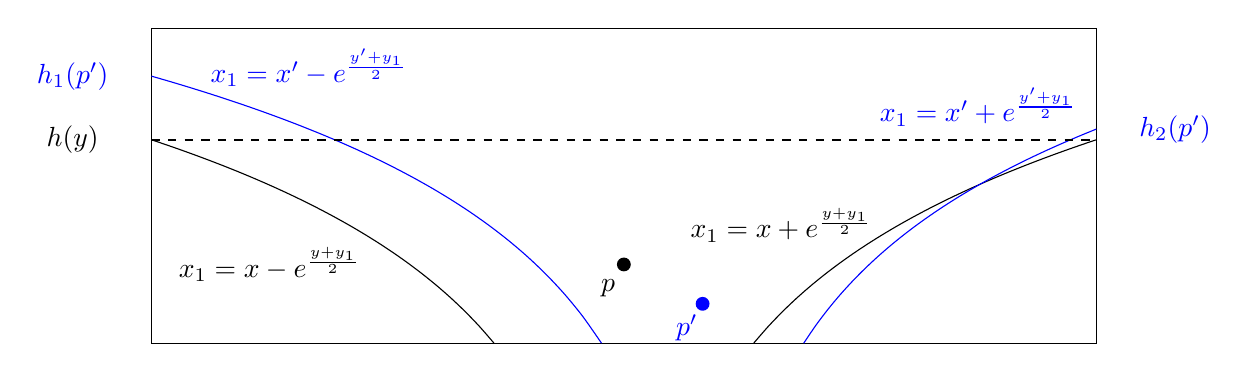
\begin{tikzpicture}
	
	%The box \Rcal_n
	\draw (-6,0) -- (6,0) -- (6,4) -- (-6,4) -- (-6,0);

    \draw node[fill, circle, inner sep=0pt, minimum size=5pt] at (0,1) {};
    \draw node at (-0.2,0.7) {$p$};
    
    \draw node[fill,blue, circle, inner sep=0pt, minimum size=5pt] at (1,0.5) {};
    \draw node at (0.8,0.2) {\color{blue}$p^\prime$};
	
	\draw[domain=1.6487:6,smooth,variable=\x,black] plot (\x, {2*ln(\x)-1});
    \draw[domain=-1.6487:-6,smooth,variable=\x,black] plot (\x, {2*ln(-\x)-1});
    \draw[domain=2.2840:6,smooth,variable=\x,blue] plot (\x, {2*ln(\x-1)-0.5});
    \draw[domain=-0.2840:-6,smooth,variable=\x,blue] plot (\x, {2*ln(1-\x)-0.5});
    
    \draw[dashed,thick,black] (-6,2.5835) -- (6,2.5835);
    
    \draw node at (-7,2.5835) {$h(y)$};
    \draw node at (-7,3.3918) {\color{blue}$h_1(p^\prime)$};
    \draw node at (7,2.7189) {\color{blue}$h_2(p^\prime)$};
    
    \draw node at (-4,3.5) {\color{blue}$x_1 = x^\prime - e^{\frac{y^\prime + y_1}{2}}$};
    \draw node at (4.5,3) {\color{blue}$x_1 = x^\prime + e^{\frac{y^\prime + y_1}{2}}$};
    \draw node at (-4.5,1) {$x_1 = x - e^{\frac{y + y_1}{2}}$};
    \draw node at (2,1.5) {$x_1 = x + e^{\frac{y + y_1}{2}}$};

\end{tikzpicture}
\caption{Schematic representation of the neighborhoods of $p$ and $p^\prime$ in $G_{\Pcal,n}(\alpha,\nu)$ when $|x-x^\prime| \le e^{\frac{y + y^\prime}{2}}$ used for the proof of Lemma \ref{lem:common_neighbors_Pcal_n}.}
\label{fig:representation_disjoint_neighborhoods_P_n}
\end{figure}

\begin{figure}[!t]
\centering
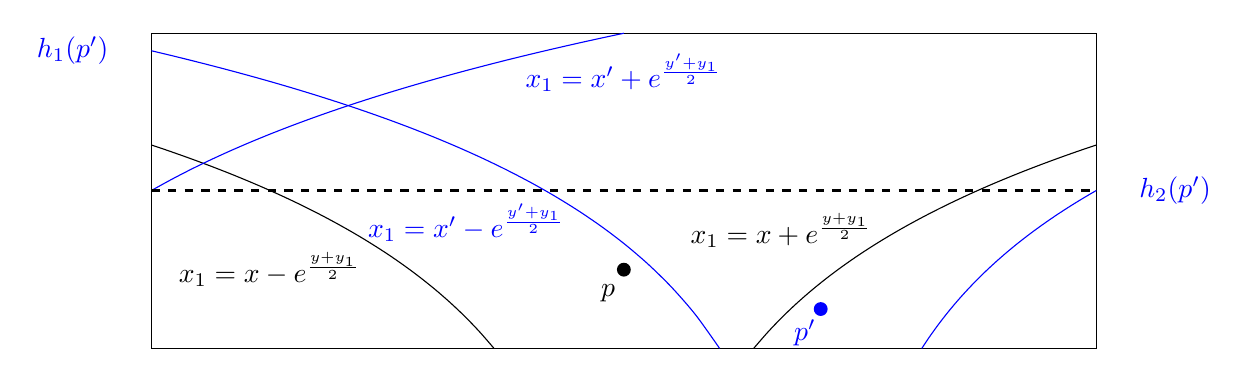
\begin{tikzpicture}
	
	%The box \Rcal_n
	\draw (-6,0) -- (6,0) -- (6,4) -- (-6,4) -- (-6,0);

    \draw node[fill, circle, inner sep=0pt, minimum size=5pt] at (0,1) {};
    \draw node at (-0.2,0.7) {$p$};
    
    \draw node[fill,blue, circle, inner sep=0pt, minimum size=5pt] at (2.5,0.5) {};
    \draw node at (2.3,0.2) {\color{blue}$p^\prime$};
	
	\draw[domain=1.6487:6,smooth,variable=\x,black] plot (\x, {2*ln(\x)-1});
    \draw[domain=-1.6487:-6,smooth,variable=\x,black] plot (\x, {2*ln(-\x)-1});
    \draw[domain=3.7840:6,smooth,variable=\x,blue] plot (\x, {2*ln(\x-2.5)-0.5});
    \draw[domain=1.2160:-6,smooth,variable=\x,blue] plot (\x, {2*ln(2.5-\x)-0.5});
    \draw[domain=0:-6,smooth,variable=\x,blue] plot (\x, {2*ln(\x+9.5)-0.5});
    
    \draw[dashed,thick,black] (-6,2.0055) -- (6,2.0055);
    
%    \draw node at (-7,2.5835) {$h(y)$};
    \draw node at (-7,3.7801) {\color{blue}$h_1(p^\prime)$};
    \draw node at (7,2.0055) {\color{blue}$h_2(p^\prime)$};
    
%    \draw[dotted,thick,black] (4.5208,2.0174) -- (4.5208,0);
%    \draw[dotted,thick,black] (4.5208,2.0174) -- (6,2.0174);
    
%    \draw node at (4.5208,-0.5) {$w_x(p,p^\prime)$};
%    \draw node at (7,2.0174) {$w_y(p,p^\prime)$};
    
    \draw node at (0,3.5) {\color{blue}$x_1 = x^\prime + e^{\frac{y^\prime + y_1}{2}}$};
    \draw node at (-2,1.6) {\color{blue}$x_1 = x^\prime - e^{\frac{y^\prime + y_1}{2}}$};
    \draw node at (-4.5,1) {$x_1 = x - e^{\frac{y + y_1}{2}}$};
    \draw node at (2,1.5) {$x_1 = x + e^{\frac{y + y_1}{2}}$};

\end{tikzpicture}
\caption{Schematic representation of the neighborhoods of $p$ and $p^\prime$ in $G_{\Pcal,n}(\alpha,\nu)$ when $e^{\frac{y + y^\prime}{2}} < |x - x^\prime| \le e^{\frac{y^\ast}{2}}\left(e^{\frac{y}{2}} + e^{\frac{y^\prime}{2}}\right)$ used for the proof of Lemma \ref{lem:common_neighbors_Pcal_n}.}
\label{fig:representation_disjoint_neighborhoods_P_n_2}
\end{figure}

\begin{figure}[!t]
\centering
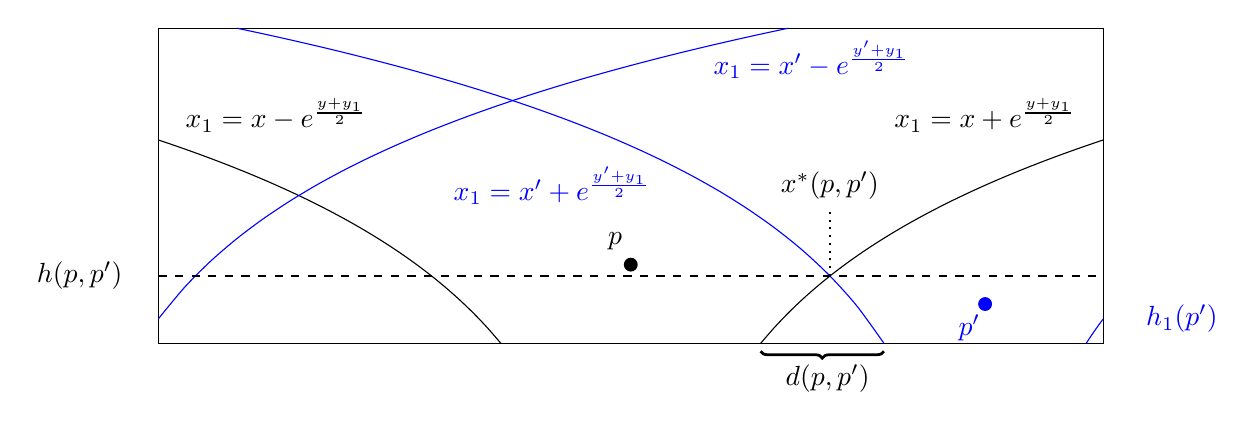
\begin{tikzpicture}
	
	%The box \Rcal_n
	\draw (-6,0) -- (6,0) -- (6,4) -- (-6,4) -- (-6,0);

    \draw node[fill, circle, inner sep=0pt, minimum size=5pt] at (0,1) {};
    \draw node at (-0.2,1.3) {$p$};
    
    \draw node[fill,blue, circle, inner sep=0pt, minimum size=5pt] at (4.5,0.5) {};
    \draw node at (4.3,0.2) {\color{blue}$p^\prime$};
	
	\draw[domain=1.6487:6,smooth,variable=\x,black] plot (\x, {2*ln(\x)-1});
    \draw[domain=-1.6487:-6,smooth,variable=\x,black] plot (\x, {2*ln(-\x)-1});
    \draw[domain=5.7840:6,smooth,variable=\x,blue] plot (\x, {2*ln(\x-4.5)-0.5});
    \draw[domain=3.2160:-5,smooth,variable=\x,blue] plot (\x, {2*ln(4.5-\x)-0.5});
    \draw[domain=2:-6,smooth,variable=\x,blue] plot (\x, {2*ln(\x+7.5)-0.5});
    
    \draw[dashed,thick,black] (-6,0.8563) -- (6,0.8563);
    
    \draw node at (-7,0.8563) {$h(p,p^\prime)$};
    \draw node at (7,0.3109) {\color{blue}$h_1(p^\prime)$};
    
    \draw [decorate,decoration={brace},line width=1pt] (3.2160,-0.1) -- (1.6487,-0.1);
    \draw node at (2.5,-0.45) {$d(p,p^\prime)$};
    
    \draw [dotted,thick] (2.5298,0.8563) -- (2.5298,1.7);
    \draw node at (2.5298,2) {$x^\ast(p,p^\prime)$};
    
%    \draw[dotted,thick,black] (4.5208,2.0174) -- (4.5208,0);
%    \draw[dotted,thick,black] (4.5208,2.0174) -- (6,2.0174);
    
%    \draw node at (4.5208,-0.5) {$w_x(p,p^\prime)$};
%    \draw node at (7,2.0174) {$w_y(p,p^\prime)$};
    
    \draw node at (2.3,3.6) {\color{blue}$x_1 = x^\prime - e^{\frac{y^\prime + y_1}{2}}$};
    \draw node at (-1,2) {\color{blue}$x_1 = x^\prime + e^{\frac{y^\prime + y_1}{2}}$};
    \draw node at (-4.5,2.9) {$x_1 = x - e^{\frac{y + y_1}{2}}$};
    \draw node at (4.5,2.9) {$x_1 = x + e^{\frac{y + y_1}{2}}$};

\end{tikzpicture}
\caption{Schematic representation of the neighborhoods of $p$ and $p^\prime$ in $G_{\Pcal,n}(\alpha,\nu)$ when $|x - x^\prime| > e^{\frac{y^\ast}{2}}\left(e^{\frac{y}{2}} + e^{\frac{y^\prime}{2}}\right)$ used for the proof of Lemma \ref{lem:disjoint_neighbors_P_n_large}.}
\label{fig:representation_disjoint_neighborhoods_P_n_3}
\end{figure}

Next we consider the number of disjoint neighbors for two points $p$ and $p^\prime$ in $G_{\Pcal,n}(\alpha,\nu)$, which we denote by $\Ncal_{\Pcal,n}(p\Delta p^\prime)$. We will distinguish between the cases where the distance between their $x$-coordinates is small and large. Due to symmetry and the fact that we have identified the left and right boundaries of the box $\Rcal_n$, we can, without loss of generality, assume that $p = (0,y)$ and $p^\prime = (x^\prime,y^\prime)$ with $x^\prime > 0$ and $y^\prime \le y$. To understand the computation it is helpful to have a picture of the different situations. Figure \ref{fig:representation_disjoint_neighborhoods_P_n} and Figure \ref{fig:representation_disjoint_neighborhoods_P_n_2} show two different situations for small distance in the $x$-coordinates, in which case the number of disjoint neighbors is small. The case where this distance is large, and the number of disjoint neighbors is expected to be large, is show in Figure \ref{fig:representation_disjoint_neighborhoods_P_n_3}. There several different quantities that are important. The are the heights $h_1(p^\prime)$ and $h_2(p^\prime)$ where, respectively, the left and right boundaries of the ball $B_{\Pcal,n}(p^\prime)$ go outside the box $\Rcal_n$. Note that when $x = 0$ then these height are the same and we denote this by $h(y)$. We also need to know the coordinates $h(p,p^\prime)$ and $x^\ast(p,p^\prime)$ of the intersection of the right boundary of the neighborhoods of $p$ with the left boundary of that of $p^\prime$. Finally we will denote by $d(p,p^\prime)$ the distance between the lower right boundary of $B_{\Pcal,n}(p)$ and the lower left of $B_{\Pcal,n}(p^\prime)$, which is positive only when the bottom parts of both neighborhoods do not intersect, compare Figures \ref{fig:representation_disjoint_neighborhoods_P_n} and \ref{fig:representation_disjoint_neighborhoods_P_n_3}. The full expressions of all these functions are given below for further reference.

\begin{align}
	h(y) &= R_n - y + 2\log\left(\frac{\pi}{2}\right) \label{eq:def_height_y_P_n}\\
	h_1(p^\prime) &= 2\log\left(x^\prime + \frac{\pi}{2}e^{\frac{R_n}{2}}\right) - y^\prime \label{eq:def_height_left_P_n} \\
	h_2(p^\prime) &= 2\log\left(\frac{\pi}{2}e^{\frac{R_n}{2}} - x^\prime\right) - y^\prime 
		\label{eq:def_height_right_P_n} \\
%	\iota_x(p,p^\prime) &= \frac{(x^\prime-x)e^{\frac{y}{2}}}{e^{\frac{y}{2}} - e^{\frac{y^\prime}{2}}}
%		\label{eq:def_x_intersection_close_boundaries}\\
%	\iota_y(p,p^\prime) &= 2\log\left(\frac{x^\prime - x}{e^{\frac{y}{2}} - e^{\frac{y^\prime}{2}}}\right)
%		\label{eq:def_y_intersection_close_boundaries}\\
	h((p,p^\prime) &= 2\log\left(\frac{|x - x^\prime|}{e^{\frac{y}{2}} + e^{\frac{y^\prime}{2}}}\right)\\
	x^\ast(p,p^\prime) &= \frac{x e^{\frac{y^\prime}{2}} + x^\prime e^{\frac{y}{2}}}{e^{\frac{y}{2}} + 	
		e^{\frac{y^\prime}{2}}},\\
	d(p,p^\prime) &= |x - x^\prime| - e^{\frac{y_\ast}{2}}\left(e^{\frac{y}{2}} + e^{\frac{y^\prime}{2}}\right) > 0,
\end{align}

We start with the result for points whose $x$-coordinates are close, which is when $d(p,p^\prime) < 0$.

\begin{lemma}\label{lem:disjoint_neighbors_P_n}
Let $p, p ^\prime \in \Rcal_n$ and let $y^\ast = \min\{y,y^\prime\}$. Then whenever $|x - x^\prime| \le e^{\frac{y^\ast}{2}}\left(e^{\frac{y}{2}} + e^{\frac{y^\prime}{2}}\right)$,
\[
	\Exp{\Ncal_{\Pcal,n}(p \Delta p^\prime)} 
	= \Omega\left(|x - x^\prime| + \left|e^{\frac{y}{2}} - e^{\frac{y^\prime}{2}}\right|\right),
\]
as $n \to \infty$.
\end{lemma}

\begin{proof}
In order to proof the result we will consider the area in between the two left boundaries of the balls $B_{\Pcal,n}(p)$ and
$B_{\Pcal,n}(p^\prime)$ up to the height $h^\ast := \min\{h(y), h_2(p^\prime)\}$. We get
\begin{align*}
	\Exp{\Pcal_n \cap \left(B_{\Pcal,n}(p) \Delta B_{\Pcal,n}(p^\prime)\right)}
	&\ge \int_0^{h^\ast} \int_{x - e^{\frac{y + y_1}{2}}}^{x^\prime - e^{\frac{y^\prime + y_1}{2}}} f_{\alpha,\nu}(x_1,y_1)
		\, dx_1 \, dy_1 \\
	&= \frac{\alpha \nu}{\pi}|x^\prime - x| \int_{0}^{h^\ast} e^{-\alpha y_1} dy_1
		+ \frac{\alpha \nu}{\pi}\left|e^{\frac{y}{2}} - e^{\frac{y^\prime}{2}}\right| \int_0^{h^\ast} 
		e^{-(\alpha-\frac{1}{2})y_1} \, dy_1\\
	&= \bigT{|x - x^\prime| + \left|e^{\frac{y}{2}} - e^{\frac{y^\prime}{2}}\right|},
\end{align*}
where we used that $h^\ast$
\end{proof}

Now we will consider the case where $|x - x^\prime| > e^{\frac{y^\ast}{2}}\left(e^{\frac{y}{2}} + e^{\frac{y^\prime}{2}}\right)$

\begin{lemma}\label{lem:disjoint_neighbors_P_n_large}
Let $p, p ^\prime \in \Rcal_n$ and let $y^\ast = \min\{y,y^\prime\}$. Then, whenever $|x - x^\prime| > e^{\frac{y^\ast}{2}}\left(e^{\frac{y}{2}} + e^{\frac{y^\prime}{2}}\right)$,
\[
	\Exp{\Ncal_{\Pcal,n}(p\Delta p^\prime)}
	\ge \left(\mu_{\alpha,\nu ,n}(B_{\Pcal,n}(p)) + \mu_{\alpha,\nu ,n}(B_{\Pcal,n}(p^\prime))\right)
		\left(1-\bigT{e^{-(\alpha - \frac{1}{2})y^\ast} - e^{-(\alpha - \frac{1}{2})R_n}}\right)
\]
as $n \to \infty$.
\end{lemma}

\begin{proof}
%Assume, without loss of generality, that $y \ge y^\prime$ and $x \le x^\prime$ and consider the boundaries of the ``balls" $B_{\Pcal,n}(p)$ and $B_{\Pcal,n}(p^\prime)$ as drawn in Figure \ref{fig:representation_disjoint_neighborhoods_P_n_3}. The left boundary of $B_{\Pcal,n}(p)$ intersects the right boundary of $B_{\Pcal,n}(p^\prime)$ if an only if
%\[
%	d(p,p^\prime) := |x - x^\prime| - e^{\frac{y_\ast}{2}}\left(e^{\frac{y}{2}} + e^{\frac{y^\prime}{2}}\right) > 0,
%\]
%which is the condition we imposed in the statement of the lemma. The $x$-coordinate of the intersection is given by
%\[
%	w(p,p^\prime) := \frac{x e^{\frac{y^\prime}{2}} + x^\prime e^{\frac{y}{2}}}{e^{\frac{y}{2}} + e^{\frac{y^\prime}{2}}},
%\]
%while the $y$-coordinate equals
%\[
%	h((p,p^\prime) := 2\log\left(\frac{|x - x^\prime|}{e^{\frac{y}{2}} + e^{\frac{y^\prime}{2}}}\right).
%\]
%In Figure \ref{fig:representation_disjoint_neighborhoods_P_n_3} this height is draw by the dashed line. 
We will prove the results by using that
\[
	\Exp{\Ncal_{\Pcal,n}(p\Delta p^\prime)} 
	\ge \int_0^{h(p,p^\prime)} \int_{-\frac{\pi}{2}e^{\frac{R_n}{2}}}^{\frac{\pi}{2}e^{\frac{R_n}{2}}} \Prob{p_1 \in B_{\Pcal,n}(p) \cup B_{\Pcal,n}(p^\prime)} f_{\alpha,\nu}(x_1,y_1) \, dx_1 \, dy_1,
\]
and computing the integral on the right. Before we proceed we show that the neighborhoods of $p$ and $p^\prime$ below $h(p,p^\prime)$ are disjoint. This is clearly true when $h(p,p^\prime) \le h_2(p^\prime)$ so suppose that $h(p,p^\prime) > h_2(p^\prime)$. Then, because we identified the right and left boundaries of the box $\Rcal_n$ the right boundary of $B_{\Pcal,n}(p^\prime)$ continues from the left boundary of the box and is described by the equation
\[
	x_1 = x^\prime + e^{\frac{y^\prime + y_1}{2}} - \pi e^{\frac{R_n}{2}}.
\]
Now, let $x_{\mathrm{right}}^\prime$ and $x_{\mathrm{left}}$ denote the $x$-coordinate of the intersection of the line $h(p,p^\prime)$ with, respectively, the right boundary of $B_{\Pcal,n}(p^\prime)$ and the left boundary of $B_{\Pcal,n}(p)$. Then
\begin{align*}
	x_{\mathrm{right}}^\prime &= x^\prime + e^{\frac{y^\prime + h(p,p^\prime)}{2}} - \pi e^{\frac{R_n}{2}}\\
	&= x^\prime + e^{\frac{h(p,p^\prime)}{2}}\left(e^{\frac{y}{2}} + e^{\frac{y^\prime}{2}}\right)
		- e{\frac{y + h(p,p^\prime)}{2}} - \pi e^{\frac{R_n}{2}}\\
	&= x^\prime + |x - x^\prime| - e{\frac{y + h(p,p^\prime)}{2}} - \pi e^{\frac{R_n}{2}}\\
	&= x - e{\frac{y + h(p,p^\prime)}{2}} + 2|x - x^\prime| - \pi e^{\frac{R_n}{2}}\\
	&\le x - e{\frac{y + h(p,p^\prime)}{2}} = x_{\mathrm{right}},
\end{align*}
and hence the neighborhoods of $p$ and $p^\prime$ below $h(p,p^\prime)$ are disjoint. It then follows that
\begin{align*}
	\Exp{\Ncal_{\Pcal,n}(p,p^\prime)} 
	&\ge \int_0^{h(p,p^\prime)} \int_{-\frac{\pi}{2}e^{\frac{R_n}{2}}}^{\frac{\pi}{2}e^{\frac{R_n}{2}}} 
		\Prob{p_1 \in B_{\Pcal,n}(p) \cup B_{\Pcal,n}(p^\prime)} f_{\alpha,\nu}(x_1,y_1) \, dx_1 \, dy_1\\
	&= \int_0^{h(p,p^\prime)} \int_{-\frac{\pi}{2}e^{\frac{R_n}{2}}}^{\frac{\pi}{2}e^{\frac{R_n}{2}}} 
		\left(\Prob{p_1 \in B_{\Pcal,n}(p)} + \Prob{p_1 \in B_{\Pcal,n}(p^\prime)}\right) 
		f_{\alpha,\nu}(x_1,y_1) \, dx_1 \, dy_1\\
	&= \left(\mu_{\alpha,\nu ,n}(B_{\Pcal,n}(p)) + \mu_{\alpha,\nu ,n}(B_{\Pcal,n}(p^\prime))\right)
		\left(1 - \frac{2\alpha \nu}{\pi}\int_{h(p,p^\prime)}^{R_n} e^{-(\alpha - \frac{1}{2})y_1} \, dy_1\right),
\end{align*}
from which the result follows since
\[
	\int_{h(p,p^\prime)}^{R_n} e^{-(\alpha - \frac{1}{2})y_1} \, dy_1 = \bigT{e^{-(\alpha - \frac{1}{2})y^\ast} - e^{-(\alpha - \frac{1}{2})R_n}}.
\]
\end{proof}

\begin{figure}
\centering
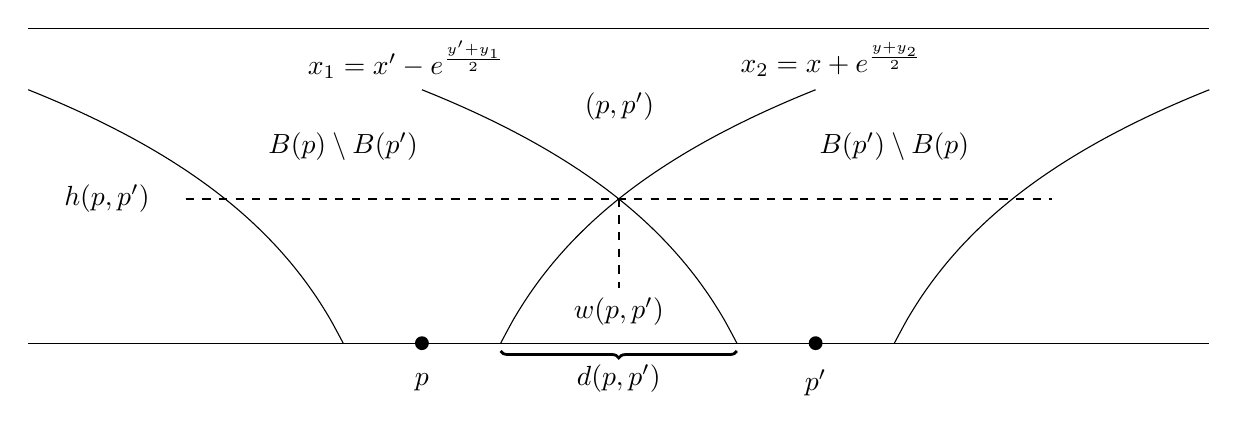
\begin{tikzpicture}
	
	%The box \Rcal_n
	\draw (-5,0) -- (10,0);
	\draw (-5,4) -- (10,4);
	
	
	\draw[domain=1:5,smooth,variable=\x,black] plot (\x, {2*ln(\x)});
    \draw[domain=-1:-5,smooth,variable=\x,black] plot (\x, {2*ln(-\x)});
    \draw[domain=6:10,smooth,variable=\x,black] plot (\x, {2*ln(\x-5)});
    \draw[domain=0:4,smooth,variable=\x,black] plot (\x, {2*ln(5-\x)});
    
    
    
    \draw node at (-1,2.5) {$B_{\Pcal}(p) \setminus B_{\Pcal}(p^\prime)$};
    
    \draw node at (-0.2,3.6) {$x_1 = x^\prime - e^{\frac{y^\prime+y_1}{2}}$};
    
    \draw node at (2.5,3) {$\Ncal_{\Pcal}(p,p^\prime)$};
    
    \draw node at (5.2,3.6) {$x_2 = x+e^{\frac{y+y_2}{2}}$};
    
    \draw node at (6,2.5) {$B_{\Pcal}(p^\prime) \setminus B_{\Pcal}(p)$};
    
    \draw[dashed,thick] (2.5,1.8326) -- (2.5,0.7);
    \draw node at (2.5,0.4) {$w(p,p^\prime)$};
    
    \draw[dashed,thick] (-3,1.8326) -- (8,1.8326);
    \draw node at (-4,1.8326) {$h(p,p^\prime)$};
    
    \draw [decorate,decoration={brace},line width=1pt] (4,-0.1) -- (1,-0.1);
    \draw node at (2.5,-0.45) {$d(p,p^\prime)$};
    
    \draw node[fill, circle, inner sep=0pt, minimum size=5pt] at (0,0) {};
    \draw node at (0,-0.5) {$p$};
    
    \draw node[fill, circle, inner sep=0pt, minimum size=5pt] at (5,0) {};
    \draw node at (5,-0.5) {$p^\prime$};
\end{tikzpicture}
\caption{Schematic representation of the neighborhoods of $p$ and $p^\prime$ in $G_{\Pcal,n}$ used for the proof of Lemma \ref{lem:common_neighbors_Pcal_n}.}
\label{fig:representation_joint_neighborhoods}
\end{figure}

Denote by $\Ncal_{\Pcal}(p,p^\prime)$ the number if common neighbors between two nodes $p$ and $p^\prime$ in $G_{\Pcal}$. 

\begin{lemma}\label{lem:common_neighbors_Pcal_n}
Let $p, p^\prime \in \Rcal_n$ and let $y_\ast = \min\{y, y^\prime\}$. Then, whenever $|x - x^\prime| > e^{\frac{y_\ast}{2}}\left(e^{\frac{y}{2}} + e^{\frac{y^\prime}{2}}\right)$,
\[
	\Exp{\Ncal_{\Pcal}(p,p^\prime)} = \frac{\nu\left(e^{\frac{y}{2}} + e^{\frac{y^\prime}{2}}\right)}{2\alpha - 1}\left(
    	\left(\frac{|x - x^\prime|}{e^{\frac{y}{2}} + e^{\frac{y^\prime}{2}}}\right)^{-(2\alpha - 1)}
        + \Theta\left(e^{-(\alpha - \frac{1}{2})R_n}\right)\right)
\]
\end{lemma}

\begin{proof}
Assume, without loss of generality, that $y \ge y^\prime$ and $x \le x^\prime$ and consider the boundaries of the ``balls" $B_{\Pcal,n}(p)$ and $B_{\Pcal,n}(p^\prime)$ as drawn in Figure \ref{fig:representation_joint_neighborhoods}. The left boundary of $B_{\Pcal,n}(p)$ intersects the right boundary of $B_{\Pcal,n}(p^\prime)$ if an only if
\[
	d(p,p^\prime) := |x - x^\prime| - e^{\frac{y_\ast}{2}}\left(e^{\frac{y}{2}} + e^{\frac{y^\prime}{2}}\right) > 0,
\]
which is the condition we imposed in the statement of the lemma. The $x$-coordinate of the intersection is given by
\[
	w(p,p^\prime) := \frac{x e^{\frac{y^\prime}{2}} + x^\prime e^{\frac{y}{2}}}{e^{\frac{y}{2}} + e^{\frac{y^\prime}{2}}},
\]
while the $y$-coordinate equals
\[
	h((p,p^\prime) := 2\log\left(\frac{|x - x^\prime|}{e^{\frac{y}{2}} + e^{\frac{y^\prime}{2}}}\right).
\]
Therefore (see Figure \ref{fig:representation_joint_neighborhoods})
\begin{align}
	\Exp{\Ncal_{\Pcal}(p,p^\prime)} 
    &= \int_{h(p,p^\prime)}^{\infty} \int_{x-e^{\frac{y+y_1}{2}}}^{w(p,p^\prime)} f_{\alpha,\nu}(x_1,y_1) \, dx_1 \, dy_1
    	\label{eq:common_neighbors_left}\\
    &\hspace{10pt}+ \int_{h(p,p^\prime)}^{\infty} \int_{w(p,p^\prime)}^{x+e^{\frac{y+y_2}{2}}} f_{\alpha,\nu}(x_2,y_2) \, dx_2 \, dy_2
    	\label{eq:common_neighbors_right}
\end{align}
We first compute \eqref{eq:common_neighbors_left}.
\begin{align*}
	&\hspace{-30pt}\int_{h(p,p^\prime)}^{\infty} \int_{x-e^{\frac{y+y_1}{2}}}^{w(p,p^\prime)} f_{\alpha,\nu}(x_1,y_1) \, dx_1 \, dy_1\\
    &= \frac{\alpha \nu}{\pi} \int_{h(p,p^\prime)}^{\infty} \left(e^{\frac{y^\prime + y_1}{2}} - (x^\prime - w(p,p^\prime))\right) 
    	e^{-\alpha y_1} \, dy_1\\
    &= \frac{\alpha \nu}{\pi}e^{\frac{y^\prime}{2}} \int_{h(p,p^\prime)}^{\infty} \left(e^{-(\alpha -\frac{1}{2})y_1} 
    	- \frac{|x - x^\prime|}{e^{\frac{y}{2}} + e^{\frac{y^\prime}{2}}} e^{-\alpha y_1}\right) \, dy_1\\
    &= \frac{\alpha \nu}{\pi(\alpha - \frac{1}{2})}e^{\frac{y^\prime}{2}}
    	\left(\frac{|x - x^\prime|}{e^{\frac{y}{2}} + e^{\frac{y^\prime}{2}}}\right)^{-(2\alpha - 1)}
    	+ \frac{\nu}{\pi}e^{\frac{y^\prime}{2}} \frac{|x - x^\prime|}{e^{\frac{y}{2}} + e^{\frac{y^\prime}{2}}}
    	\left(\frac{|x - x^\prime|}{e^{\frac{y}{2}} + e^{\frac{y^\prime}{2}}}\right)^{-2\alpha} \\
    &= \frac{\nu}{2\alpha - 1} e^{\frac{y^\prime}{2}}
    	\left(\frac{|x - x^\prime|}{e^{\frac{y}{2}} + e^{\frac{y^\prime}{2}}}\right)^{-(2\alpha - 1)}.
\end{align*}
In a similar way we get that \eqref{eq:common_neighbors_right} equals
\[
	\frac{\nu}{2\alpha - 1} e^{\frac{y}{2}}
    	\left(\frac{|x - x^\prime|}{e^{\frac{y}{2}} + e^{\frac{y^\prime}{2}}}\right)^{-(2\alpha - 1)}.
\]
Therefore we conclude that
\[
	\Exp{\Ncal_{\Pcal}(p,p^\prime)} = \frac{\nu\left(e^{\frac{y}{2}} + e^{\frac{y^\prime}{2}}\right)}{2\alpha - 1}
    	\left(\frac{|x - x^\prime|}{e^{\frac{y}{2}} + e^{\frac{y^\prime}{2}}}\right)^{-(2\alpha - 1)}.
\]
\end{proof}

\subsection{Joint distributions in $G_{\Pcal,n}(\alpha,\nu)$}

To ease notations we introduce the following short-hand notation for the conditional joint degree distribution
\[
	\varphi_{p,p^\prime}(k,k^\prime) 
	:= \Prob{D_{\Pcal,n}(p) = k, D_{\Pcal,n}(p^\prime) = k^\prime}.
\]

\begin{lemma}\label{lem:joint_degree_distribution_shift}
Let $\alpha > \frac{1}{2}$, $\nu > 0$, $k_n \to \infty$ and fix $\varepsilon > 0$. Then for any fixed $i, j, i^\prime, j^\prime \in \mathbb{Z}$ and $p, p^\prime \in \Kcal_{\varepsilon}(k_n)$ such that $\Exp{\left|\Ncal_{\Pcal,n}(p,p^\prime)\right|} \ge k_n^{\varepsilon}$,
\[
	\varphi_{p,p^\prime}(k_n + i,k_n + i^\prime) 
	= (1 + o(1))\varphi_{p,p^\prime}(k_n + j,k_n + j^\prime)  \pm e^{-\Omega(k_n^\varepsilon)}.
\]
\end{lemma}

\begin{proof}

Define
\begin{align*}
	X_n = \left|\Ncal_{\Pcal,n}(p) \setminus \Ncal_{\Pcal,n}(p^\prime)\right|,\\
	Y_n = \left|\Ncal_{\Pcal,n}(p) \cap \Ncal_{\Pcal,n}(p^\prime)\right|,\\
	Z_n = \left|\Ncal_{\Pcal,n}(p^\prime) \setminus \Ncal_{\Pcal,n}(p)\right|.
\end{align*}
Then it follows that $X_n$, $Y_n$ and $Z_n$ are independent Poisson random variables satisfying $\Exp{X_n} + \Exp{Y_n} = \mu_{n}(B_{\Pcal,n}(p))$ and $\Exp{Z_n} + \Exp{Y_n} = \mu_{n}(B_{\Pcal,n}(p^\prime))$ while
\begin{align*}
	\varphi(p,p^\prime,k_n + i,k_n + i^\prime) &= \Prob{X_n + Y_n = k + i, Z_n + Y_n = k + i^\prime}\\
	&= \sum_{\ell = 0}^\infty \Prob{Y_n = \ell} \Prob{X_n = k + i - \ell, Z_n = k + i^\prime - \ell} \\
	&= \sum_{\ell = 0}^\infty \Prob{Y_n = \ell} \Prob{X_n = k + i - \ell} \Prob{Z_n = k + i^\prime - \ell}.
\end{align*}
Next define $\delta_n = k_n^{-\frac{1-\varepsilon}{2}}$, let $n$ be large enough such that $0 < \delta_n < 1$ and note that by a Chernoff bound,
\[
	\Prob{|X_n - \Exp{X_n}| > \delta_n \Exp{X_n}} = \bigO{e^{-\frac{\delta_n^2}{4(1+\delta_n)} \Exp{X_n}}},
\]
and similar for $Y_n$ and $Z_n$. Finally, we define
\begin{align*}
	L_X &= \left\{\ell : (1 - \delta_n) \Exp{X_n} \le k + i - \ell \le (1+\delta_n)\Exp{X_n}\right\} \\
	L_y &= \left\{\ell : (1 - \delta_n) \Exp{Y_n} \le \ell \le (1+\delta_n)\Exp{Y_n}\right\}\\
	L_Z &= \left\{\ell : (1 - \delta_n) \Exp{Z_n} \le k + i^\prime - \ell \le (1+\delta_n)\Exp{Z_n}\right\}
\end{align*}
We will now make distinguish between the cases $\Exp{Y_n} \le k_n/2$ and $\Exp{Y_n} > k_n/n$. 

Let us first assume that $\Exp{Y_n} \le k_n/2$. Then, since $p,p^\prime \in \Kcal_{\varepsilon}(k_n)$, $\mu_{\alpha,\nu,n}(B_{\Pcal,n}(p)) = \Theta(e^{\frac{y}{2}}) = \Theta(k_n)$ by Lemma \ref{lem:average_degree_P_n}. Therefore, $\Exp{X_n} \ge \Omega(k_n)$ and hence
\[
	\Prob{|X_n - \Exp{X_n}| > \delta_n \Exp{X_n}} = \bigO{e^{-\frac{\delta_n^2}{4(1+\delta_n)} \Exp{X_n}}} = e^{-\Omega(k_n^\varepsilon)}.
\]
In particular, this implies
\begin{align*}
	&\hspace{-30pt}\sum_{\ell \notin L_X} \Prob{Y_n = \ell} \Prob{X_n = k + i - \ell} 
			\Prob{Z_n = k + i^\prime - \ell}\\
	&= \bigO{\Prob{|X_n - \Exp{X_n}| > \delta_n \Exp{X_n}}} = e^{-\Omega(k_n^\varepsilon)},
\end{align*}
Finally we note that, for $\ell \in L_X$, we have
\begin{equation}\label{eq:fraction_degree_prob}
	\frac{\Prob{X_n = k + i - \ell}}{\Prob{X_n = k + j - \ell}} = \Exp{X_n}^{i - j} \frac{(k + j - \ell)!}{(k + i - \ell)!}
	\le (1 + \delta_n)^{2|i - j|}.
\end{equation}
and observe that we have similar results for $Z_n$. Therefore,
\begin{align*}
	&\hspace{-30pt}\sum_{\ell \in L_X \cap L_Z} \Prob{Y_n = \ell} \Prob{X_n = k + i - \ell} 
		\Prob{Z_n = k + i^\prime - \ell} \\
	&\le (1+\delta_n)^{2(j-i) + 2(j^\prime - i^\prime)} \sum_{\ell \in L_x \cap L_Z} 
			\Prob{Y_n = \ell} \Prob{X_n = k + j - \ell} \Prob{Z_n = k + j^\prime - \ell}\\
	&= (1+o(1))(1+\delta_n)^{2|i-j| + 2|i^\prime - j^\prime|}\Prob{D_p = k_n + j, D_{p^\prime} = k_n + j^\prime}\\
	&= (1+o(1))\Prob{D_p = k_n + j, D_{p^\prime} = k_n + j^\prime}
\end{align*}
and hence
\begin{align*}
	\Prob{D_p = k_n + i, D_{p^\prime} = k_n + i^\prime}
	&= (1+o(1))\Prob{D_p = k_n + j, D_{p^\prime} = k_n + j^\prime} + e^{-\Omega(k_n^\varepsilon)}.
\end{align*}

Now assume that $\Exp{Y_n} > k_n/2$. Then, since $\Exp{\left|\Ncal_{\Pcal,n}(p,p^\prime)\right|} \ge k_n^{\varepsilon}$ it follows that $\Exp{X_n} = \Omega(k_n^\varepsilon)$ or $\Exp{Z_n} = \Omega(k_n^\varepsilon)$. Without loss of generality we assume that $\Exp{X_n} = \Omega(k_n^\varepsilon)$. Similar to \eqref{eq:fraction_degree_prob} we have for $Y_n$
\[
	\frac{\Prob{Y_n = \ell}}{\Prob{Y_n = \ell + j^\prime - i^\prime}} \le (1 + \delta_n)^{2(|i^\prime - j^\prime|)}.
\]
Using similar computations as above we then have
\begin{align*}
	&\hspace{-30pt}\Prob{D_p = k_n + i, D_{p^\prime} = k_n + i^\prime} \\
	&= \sum_{\ell \in L_X \cap L_Y} \Prob{Y_n = \ell} \Prob{X_n = k + i - \ell}
		\Prob{Z_n = k + i^\prime - \ell}  + e^{-\Omega(k_n^\varepsilon)}\\
	&= (1+o(1))\Prob{D_p = k_n + j, D_{p^\prime} = k_n + j^\prime} + e^{-\Omega(k_n^\varepsilon)}.
\end{align*}

\end{proof}


\begin{lemma}\label{lem:joint_degree_distribution_P_n}
Let $\alpha > \frac{1}{2}$, $\nu > 0$ and fix $\varepsilon > 0$. Then for any $p, p^\prime \in \Kcal_{\varepsilon}(k)$ such that $|x - x^\prime| \ge k^{1 + \varepsilon}$, as $n \to \infty$,
\begin{align*}
	&\hspace{-30pt}\Prob{D_{\Pcal ,n}(p) = k - |B_{\Pcal,n}(p) \cap \{p^\prime\}|, 
		D_{\Pcal, n}(p^\prime) = k - |B_{\Pcal,n}(p^\prime) \cap \{p\}|}\\
	&= (1 + o(1)) \Prob{D_{\Pcal ,n}(p) = k} \Prob{D_{\Pcal ,n}(p^\prime) = k} + k^{-\omega(1)}.
\end{align*}
\end{lemma}

\begin{proof}
This is a direct consequence of Lemma~\ref{lem:joint_degree_distribution_shift} and Lemma~\ref{lem:joint_distribution_Poisson}.
\end{proof}

%\begin{lemma}
%Let $\alpha > \frac{1}{2}$, $\nu > 0$ and $\{k_n\}_{n \ge 1}$ be a non-decreasing sequence such that $k_n = \bigO{n^{\frac{1}{2\alpha + 1}}}$. Then, as $n \to \infty$,
%\begin{align*}
%	\Exp{N_{\Pcal,n}(k_n)^2} = (1 + o(1)) \Exp{N_{\Pcal,n}(k_n)}^2
%\end{align*}
%\end{lemma}


\section{Some results for random variables}

We start with the following concentration result which follows from~\cite[Theorem 4]{freedman1973another}, together with the note directly after it.

\begin{lemma}\label{lem:general_concentration_sum_indicators}
Let $X_n$ be a sum of $n$, possibly dependent, indicators and $c > 0$. Then
\[
	\Prob{|X_n - \Exp{X_n}| > c \Exp{X_n}} \le 2 e^{-\frac{c \Exp{X_n}}{2}}.
\]
\end{lemma}

Let $H(x) = x\log(x) - x + 1$. Then by a Chernoff bound, see for instance \cite[Lemma 1.2]{penrose2003random},
\begin{align*}
	&\Prob{\Po(\lambda) \ge k} \le e^{-\lambda H(k/\lambda)} \quad \text{for all } k \ge \lambda\\
	&\Prob{\Po(\lambda) \le k} \le e^{-\lambda H(k/\lambda)} \quad \text{for all } k \le \lambda.
\end{align*}
Note that $H(x) \le (x-1)^2/2$ for all $0 \le x \le 1$. Therefore, 
\begin{align*}
	\Prob{\left|\mathrm{Po}(\lambda) - \lambda\right| \ge x} \ge 1 - e^{-\lambda H(1 - x/\lambda)} - e^{-\lambda H(1 + x/\lambda)}
\end{align*}
 $\Pee(X >k) \leq e^{-\mu H(\frac{k}{\mu})}$ and for $k<\mu$, $\Pee(X< k) \leq e^{-\mu H(\frac{k}{\mu})}$, where $H(x) = x\ln x -x+1$, \cite{Penrose2003}), it follows that $\Pee(N \in [n-c\sqrt{n\log n},n+c\sqrt{n\log n}]) \geq 1-e^{-n H(\frac{n-c\sqrt{n\log n}}{n})}-e^{-nH(\frac{n+c\sqrt{n \log n}}{n})} \geq  1-2e^{-n \frac{c^2 n \log n}{n^2}} = 1-2e^{-c^2\log n}=1-2n^{-c^2}$ (where we have used that $H(x) = (x-1)^2$ for $x$ close to 1)

By a Chernoff bound we have
\begin{equation}\label{eq:def_chernoff_bound_poisson}
	\Prob{\left|\mathrm{Po}(\lambda) - \lambda\right| \ge x} \le 2e^{-\frac{x^2}{2(\lambda + x)}}.
\end{equation}
In particular, if $\lambda_n \to \infty$, then, for any $0 < \varepsilon < 1$,
\[
	\Prob{\left|\mathrm{Po}(\lambda_n) - \lambda_n\right| \ge \lambda_n^{\frac{1+\varepsilon}{2}}} \le 2e^{-\frac{\lambda_n^\varepsilon}{2\left(1 + \lambda_n^{-(1 - \varepsilon)/2}\right)}}
	= \bigO{e^{-\lambda_n^\varepsilon}}.
\]

\PvdH{The results below still need to be converted to match style and notation.}
\begin{lemma}\label{lem:Poissonstab}
Let $k_n$ be a sequence of natural numbers, $\mu_n^{(1)}, \mu_n^{(2)}$ sequences of positive real numbers and $X_n = \mathrm{Po}(\mu_n^{(1)})$ be a Poison random variable with mean $\mu_n^{(1)}$. In addition, Let $h_n = \smallO{\sqrt{\frac{k_n}{\log k_n}}}$, $c > 0$ and assume that $k_n-\mu_n^{(2)} = \mu_n^{(1)}+a_n$ with $a_n \in [-c\sqrt{k_n\log k_n},c\sqrt{k_n\log k_n}]$ and $\mu_n^{(1)}=\Theta(k_n)$. 
Then, as $n \to \infty$,
\[
	\Prob{X_n = k_n - \mu_n^{(3)}} \sim \Prob{X_n = k_n - \mu_n^{(2)} + h_n}.
\]
\end{lemma}
\begin{proof}
	Firstly, we upper bound the ratio:
	\begin{align*}
	\frac{\Pee(Po(\mu_1)=k-\mu_3)}{\Pee(Po(\mu_1)=k-\mu_3 +h)} &= \mu_1^{-h} \frac{(k-\mu_3+h)!}{(k-\mu_3)!}  \leq \mu_1^{-h} (k-\mu_3+h)^h\\
	 &= \mu_1^{-h} (\mu_1+g+h)^h = (1+\frac{g+h}{\mu_1})^h \leq e^{\frac{(g+h)h}{\mu_1}}
	\end{align*}
	which tends to 1 by the assumptions on $g,h$ and $\mu_1$.
	
	Similarly, the ratio can be lower bounded by 1:
	\begin{align*}
	\frac{\Pee(Po(\mu_1)=k-\mu_3)}{\Pee(Po(\mu_1)=k-\mu_3 +h)} &= \mu_1^{h} \frac{(k-\mu_3+h)!}{(k-\mu_3)!}  \geq \mu_1^{-h} (k-\mu_3)^h\\
	 &= \mu_1^{-h} (\mu_1+g)^h = (1+\frac{g}{\mu_1})^h \geq 1 
	\end{align*}
\end{proof}

\begin{lemma}[Near independence of Poisson variables]\label{lem:joint_distribution_Poisson}
	Let $X_1, X_2, X_3$ be independent Poisson random variables with expectations $\lambda_1, \lambda_2, \lambda_3$ (where everything depends on $n$, i.e. formally a sequence of such random variables). Let $k=k_n \in \N_0$ be a sequence of natural numbers. Let $C>0$.
	
	If $\lambda_3 \leq  k^{1-\epsilon}$ (for any $\epsilon>0$) and $\lambda_1, \lambda_2 = \Theta(k)$, %we will later pick $\epsilon= \delta(2\alpha-1)$;
	%$\mu_3 \ll \mu_1 \sim \mu_2 \sim k$ and $(\frac{\mu_1}{\mu_1+\mu_3})^k, (\frac{\mu_2}{\mu_2+\mu_3})^k \sim e^{-\mu_3}$, 
	then (as $n \rightarrow \infty$) 
	$$\Pee(X_1+X_3=X_2+X_3=k) =(1+o(1)) \Pee(X_1+X_3=k)\Pee(X_2+X_3=k)+O(k^{-C})$$
	 %$k \sim \mu_1+\mu_3 \sim \mu_2+\mu_3$, $\mu_3 \ll \mu_1$ and $\mu_3 \ll \mu_2$
\end{lemma}
\begin{proof}
Let $C>0$ and $c = \sqrt{C}$.
From $\lambda_3 \leq k^{1-\epsilon}$ it follows by the Chernov bound for Poisson random variables that $\Pee(|X_3-\lambda_3| \geq c\sqrt{k^{1-\epsilon} \log k}) \leq k^{-c^2} = k^{-C}$. Note that $h:= c\sqrt{k^{1-\epsilon} \log k} = o(\sqrt{\frac{k}{\log k}})$.

Conditioning on the value of $X_3$ and then separating the values according to the event $A$ that $X_3 \in [\lambda_3-h,\lambda_3 +h]$ gives
\begin{align*}
\Pee( X_1+X_3 = X_2 + X_3 =k) &= \sum_{k_3 \in [\lambda_3-h,\lambda_3+h]} \Pee(X_1=X_2=k-k_3)\Pee(X_3=k_3) \\
 \\ &\qquad \qquad+ \sum_{k_3 \not \in [\lambda_3-h,\lambda_3+h]} \Pee(X_1=X_2=k-k_3)\Pee(X_3=k_3) \\
&=\sum_{k_3 \in [\lambda_3-h,\lambda_3+h]} \Pee(X_1=k-k_3)\Pee(X_2=k-k_3)\Pee(X_3=k_3) + k^{-C}
\end{align*}
where we have used the independence of $X_1$ and $X_2$ in the last line. Now applying lemma E2 \GR{please replace with proper reference)} and then summarizing all the terms results in
\begin{align*}
=\sum_{k_3 \in [\lambda_3-h,\lambda_3+h]} (1+o(1))\Pee(X_1=k-\lambda_3)\Pee(X_2=k-\lambda_3)\Pee(X_3=k_3) +k^{-C} \\
= (1+o(1)) \Pee( X_1 =k- \lambda_3 ) \Pee(  X_2 = k-\lambda_3) +k^{-C}
\end{align*}
On the other hand, again by conditioning on the event $A$,
\begin{align*}
\Pee(X_1+X_3=k) = \sum_{k_3 \in [\lambda_3-h,\lambda_3+h]} \Pee(X_1=k-k_3)\Pee(X_3 = k_3)+\Pee(X_1+X_3=k|A^c)\Pee(A^c)\\
 = (1+o(1))\Pee(X_1=k- \lambda_3)\Pee(A) +k^{-C} \\
 =(1+o(1))\Pee(X_1=k-\lambda_3)+k^{-C}
\end{align*}
and likewise
\begin{align*}
\Pee(X_2+X_3=k)
 = (1+o(1))\Pee(X_2=k- \lambda_3) +k^{-C}
\end{align*}
Therefore, their product has the form
\begin{align*}
&\Pee(X_1+X_3=k)\Pee(X_2+X_3=k) \\
&= (1+o(1))\Pee(X_1=k-\lambda_3)\Pee(X_2=k-\lambda_3)+O(k^{-C})
\end{align*}
We conclude that both sides in the claim agree.
\end{proof}
\end{appendices}